
\noindent In this chapter, we will explore the first question: How to form a distribution aware method of compressing binary neural networks. As illustrated in Figure \ref{fig:alphabetadiagram} that changes in the binarization function can influence it's ability to detect portions of an image more accurately.

\begin{figure}[h]
\centering
           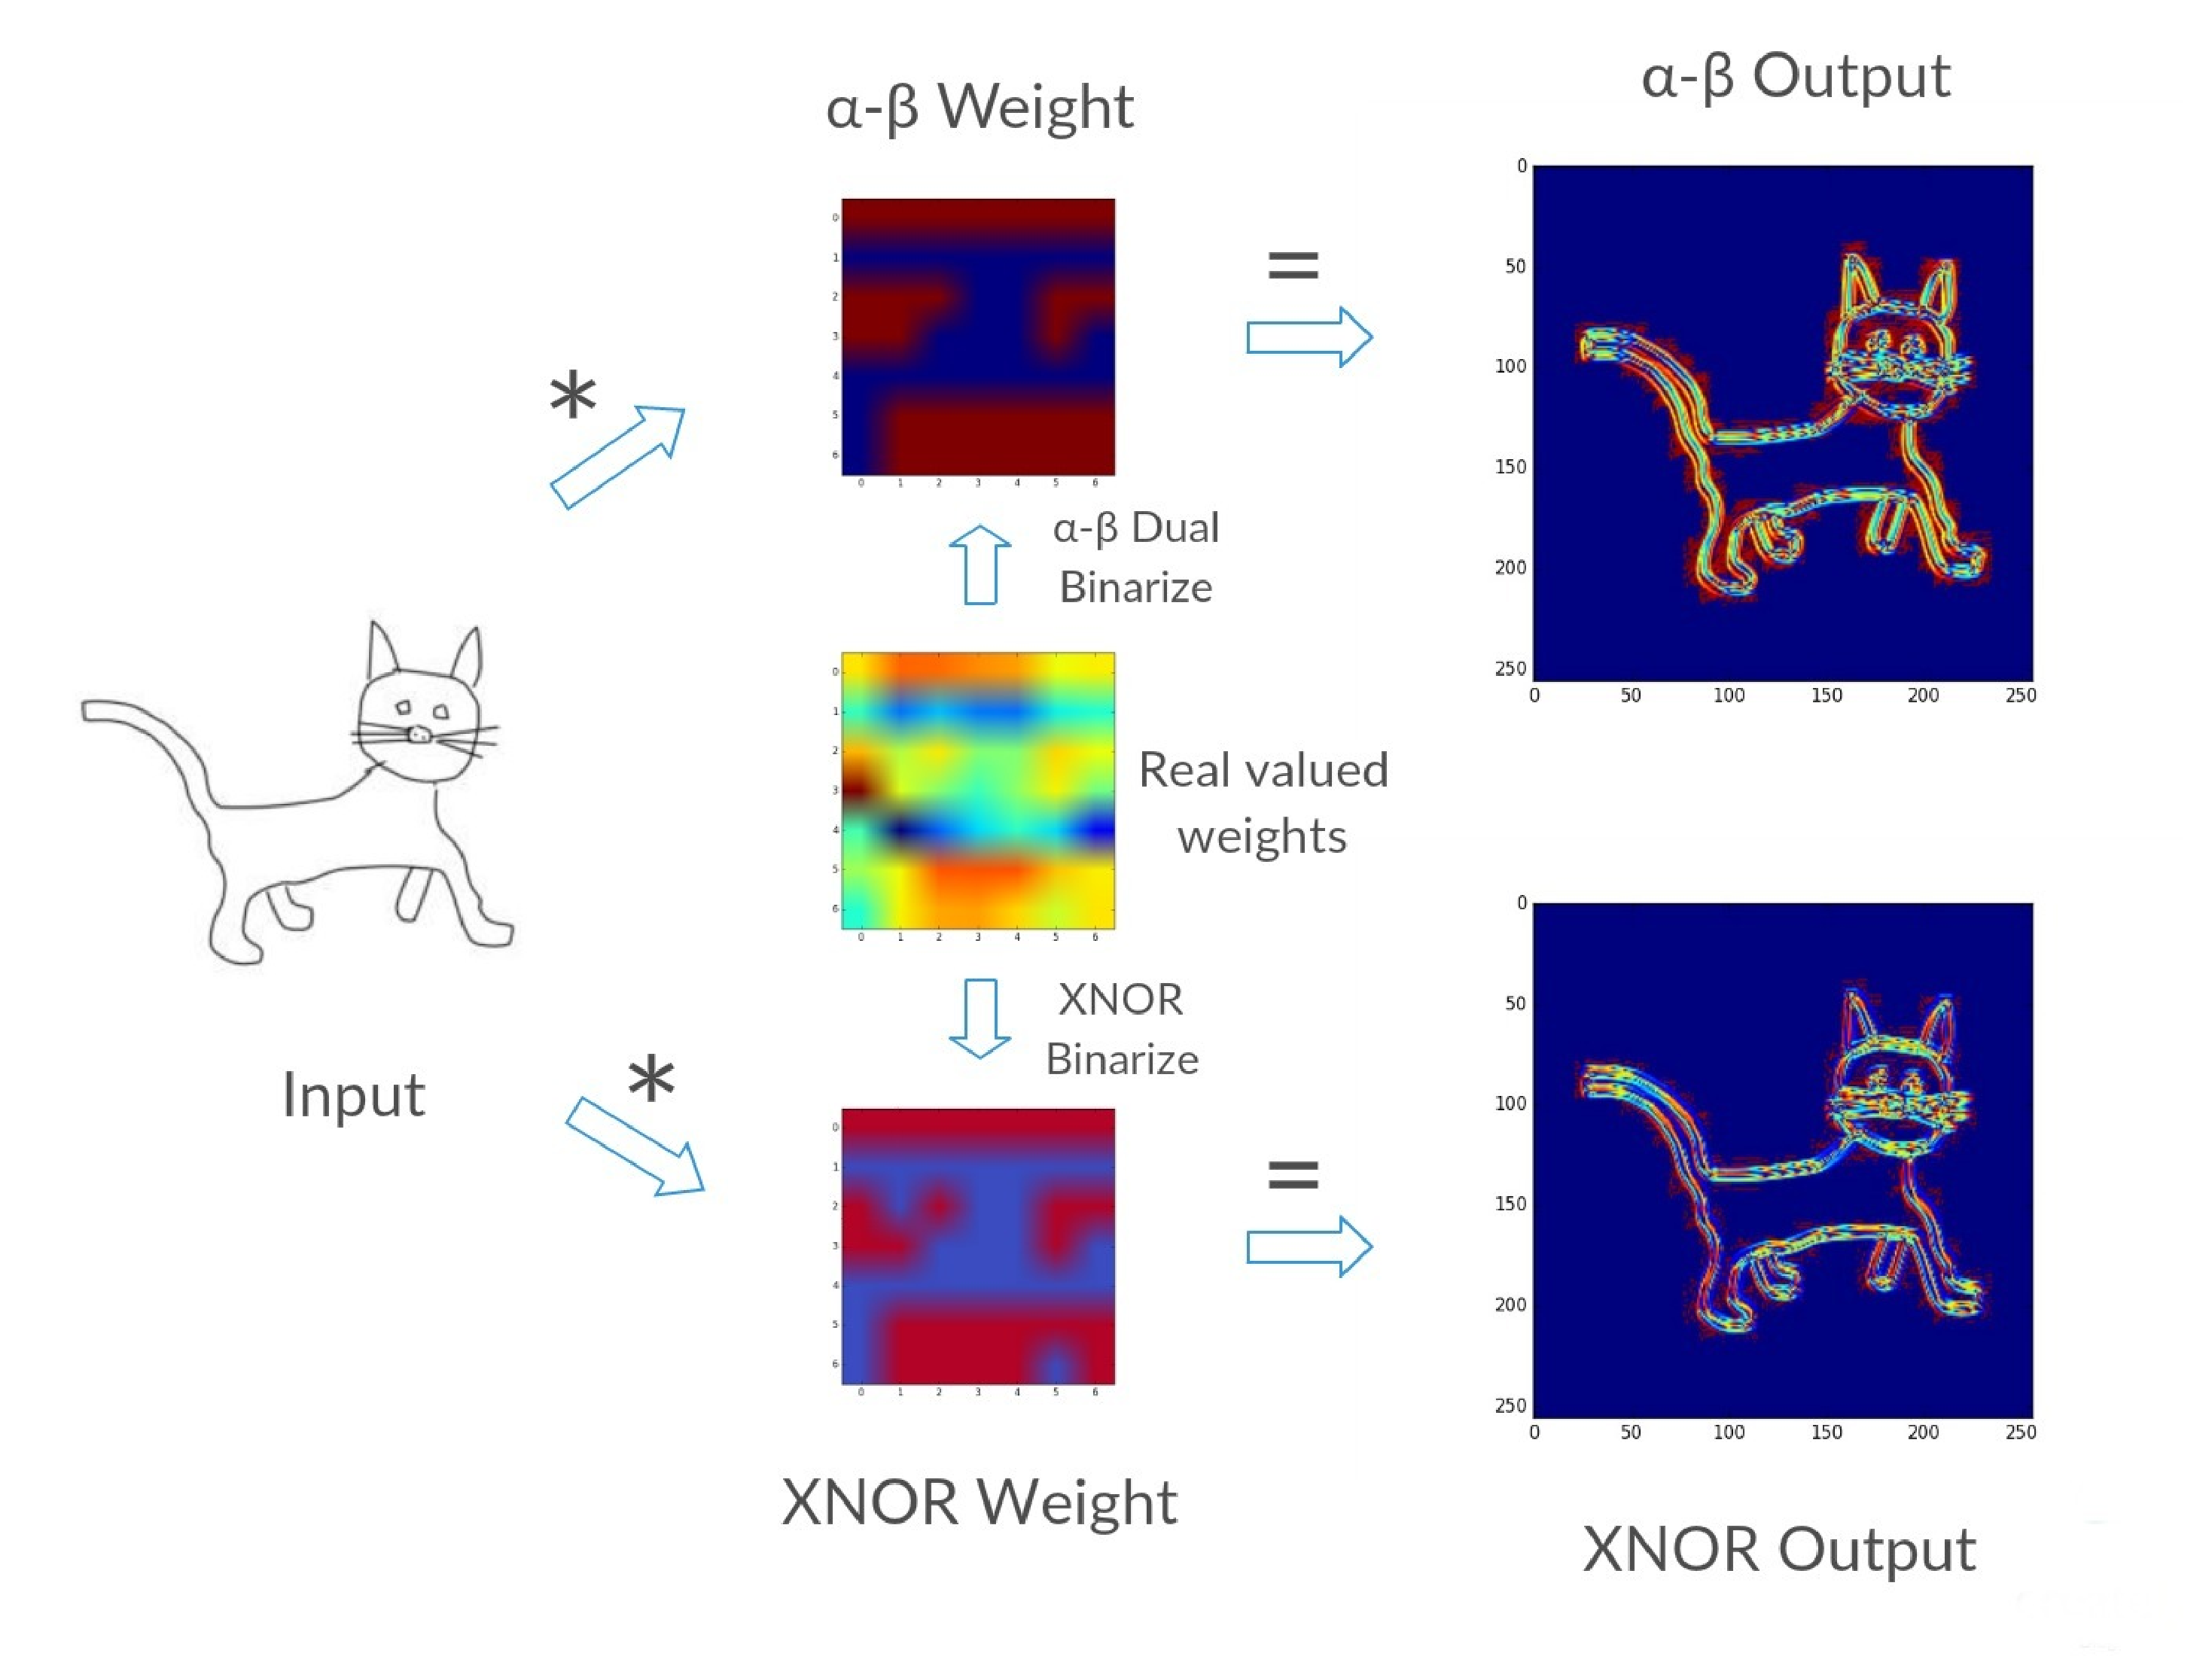
\includegraphics[width=0.45\textwidth]{figures/MainDiagram-CVPR.pdf}
           \caption{An example sketch passing through a convolutional layer filter, with the real-valued filter shown alongside corresponding $\alpha$-$\beta$ and XNOR-Net filters. Orange signifies the highest response areas. We can see that DAB-Net has significantly better responses when compared to XNOR-Net}
        \label{fig:alphabetadiagram}
\end{figure}

\section{Representational Power of Binary Networks} 

\noindent Many recent works in network compression involve higher bit weight quantization using two or more bits \cite{zhou2017inq,li2016ternary,li2016ternary} instead of binarization, arguing that binary representations would not be able to approximate full-precision networks. In light of this, we explore whether the representational power that binary networks can offer is theoretically sufficient to get similar representational power as full-precision networks.\\

\noindent Rolnick \etal \cite{lin2017does,rolnick2017power} have done extensive work in characterizing the expressiveness of neural networks. They claim that due to the nature of functions - that they depend on real-world physics, in addition to mathematics - the seemingly huge set of possible functions could be approximated by deep learning models. From the Universal Approximation Theorem \cite{cybenko1989approximation}, it is seen that any arbitrary function can be well-approximated by an Artificial Neural Network; but \textit{cheap learning}, or models with far fewer parameters than generic ones, are often sufficient to approximate multivariate monomials - which are a class of functions with practical interest, occurring in most real-world problems.\\

\noindent We can define a binary neural network having $k$ layers with activation function $\sigma(x)$  and consider how many neurons are required to compute a multivariate monomial $p(x)$ of degree $d$. The network takes an $n$ dimensional input $\mathbf{x}$, producing a one dimensional output $p(x)$. We define $B_k(p,\sigma)$ to be the minimum number of binary neurons (excluding input and output) required to approximate $p$, where the error of approximation is of degree at least $d+1$ in the input variables. For instance, $B_1(p,\sigma)$ is the minimal integer $m$ such that:
$$\sum_{j=1}^m w_j \sigma\left(\sum_{i=1}^n a_{ij} x_i\right) = p(x) + \mathcal{O}(x_1^{d + 1} + \ldots + x_n^{d + 1}).$$ 
Any polynomial can be approximated to high precision as long as input variables are small enough \cite{lin2017does}. Let $B(p, \sigma) = \min_{k \geq 0} B_k(p, \sigma)$.

\begin{theorem}
\label{theorem:binaryrepresentation}
For $p(\mathbf{x})$ equal to the product $x_1x_2\cdots x_n$, and for any $\sigma$ with all nonzero Taylor coefficients, we have one construction of a binary neural network which meets the condition
\begin{equation}
B_k(p, \sigma) = \mathcal{O}\left(n^{(k-1)/k}\cdot 2^{n^{1/k}}\right).\label{eqn:constantlayers}
\end{equation}

Proof of the above can be found in the appendix A. 
\end{theorem}

\noindent Conjecture III.2. of Rolnick \etal \cite{rolnick2017power} says that this bound is approximately optimal. If this conjecture is true, weight-binarized networks would have the same representational  power as full-precision networks, but with finite (1-bit) precision. Another case would be 2 layer network, where we can say a binary network requires the same number of neurons as a full-precision network, $2^n$. 

\begin{theorem}
For any desired accuracy $\epsilon>0$, there exists a binary neural network $B_1(p,\sigma)$ that can compute the function $p(x)$ using a single hidden layer of $2^n$ binary-weighted neurons.

Proof of the above can be found in the appendix A.
\end{theorem}

\noindent The above theorem shows that any neural network that can be represented as a multivariate polynomial function is considered as a simplified model with ELU-like activations, using continuously differentiable layers - so pooling layers are excluded as well. While there can exist a deep binary-weight network that can possibly approximate polynomials similar to full precision networks, it does say that such a representation would be efficiently obtainable through Stochastic Gradient Descent. Also, this theorem assumes only weights are binarized, not the activations. Activation binarization typically loses a lot of information and might not be a good thing to do frequently. However, this insight motivates the fact that more investigation is needed into approximating networks through binary network structures.

\section{Distribution-Aware Binarization}

\noindent We have so far established that binary representations are possibly sufficient to approximate a polynomial with similar numbers of neurons as a full-precision neural network. We now investigate the question - What is the most general form of binary representation possible? In this section, we derive a generalized distribution-aware formulation of binary weights, and provide an efficient implementation of the same. We consider models binarized with our approach as DAB-Nets (Distribution Aware Binarized Networks).\\

\noindent We model the loss function layer-wise for the network. We assume that inputs to the convolutional layers are binary - i.e. belong to $\{+1, -1\}$, and find constants $\alpha$ and $\beta$ (elaborated below) as a general binary form for layer weights. These constants are calculated from the distribution of real-valued weights in a layer - thus making our approach \textit{distribution-aware}. 

\subsection{Derivation}
\noindent Without loss of generality, we assume that $\mathbf{W}$ is a vector in $R^{n}$ , where $n = c\cdot w\cdot h$.
We attempt to binarize the weight vector $\mathbf{W}$ to $\widetilde{\mathbf{W}}$ which takes a form similar to this example - $[\alpha \alpha... \beta \alpha \beta]$. Simply put, $\widetilde{\mathbf{W}}$ is a vector consisting of scalars $\alpha$ and $\beta$, the two values forming the binary vector. We represent this as $\widetilde{\mathbf{W}} = \alpha \mathbf{e} + \beta \mathbf{(1-e)}$ where $\mathbf{e}$ is a vector such that $\mathbf{e} \in \{0,1\}^n \ni \mathbf{e} \neq 0$ and $\mathbf{e} \neq 1$.  We define $K$ as $\mathbf{e}^T\mathbf{e}$ which represents the number of ones in the $\mathbf{e}$ vector. Our objective is to find the best possible binary approximation for $\mathbf{W}$. We set up the optimization problem as: $$\widetilde{\mathbf{W}}^\ast = \underset{\widetilde{\mathbf{W}}}{\mathrm{argmin}}\mid\mid \mathbf{W}-\widetilde{\mathbf{W}}\mid\mid^{2}$$ We formally state this as the following: \\

%\begin{theorem}
\label{approx}
{\it The optimal binary weight vector $\widetilde{\mathbf{W}}^\ast$ for any weight vector $\mathbf{\mathbf{W}}$ which minimizes the approximate-error function $\mathbf{J} = \mid\mid \mathbf{W}-\widetilde{\mathbf{W}}\mid\mid^{2}$ can be represented as: %in terms of scalar parameters $\alpha$, $\beta$ and vector $e$ as: 
$$\widetilde{\mathbf{W}}^\ast = \alpha \mathbf{e} + \beta \mathbf{(1-e)}  \; where\\$$
$$ \alpha =\frac{\mathbf{W}^{T}\mathbf{e}}{K} \;, \; \beta = \frac{\mathbf{W}^{T}\mathbf{(1-e)}}{n-K} $$ for a given $K$. That is, given a $K$, the optimal selection of $\mathbf{e}$ would correspond to either the $K$ smallest weights of $\mathbf{W}$ or the $K$ largest weights of $\mathbf{W}$. 

The best suited $K$, we calculate the value of the following expression for every value of $K$, giving us an $\mathbf{e}$, and maximize the expression: $$  \mathbf{e}^\ast  = \underset{\mathbf{e}}{\mathrm{argmax}}  (\frac{\mid\mid\mathbf{\mathbf{W}}^T\mathbf{e}\mid\mid^2}{K}+\frac{\mid\mid\mathbf{W}^T\mathbf{(1-e)}\mid\mid^2}{n-K}) \\$$
A detailed proof of the above can be found in the appendix A.}
\\\\
\noindent The above representation shows the values obtained for $\mathbf{e}$, $\alpha$ and $\beta$ are the optimal approximate representations of the weight vector $\mathbf{W}$. The vector $\mathbf{e}$, which controls the number and distribution of occurrences of $\alpha$ and $\beta$, acts as a mask of the top/bottom $K$ values of $\mathbf{W}$. We assign $\alpha$ to capture the greater of the two values in magnitude. Note that the scaling values derived in the XNOR formulation, $\alpha$ and $-\alpha$, are a special case of the above, and hence our approximation error is at most that of the  XNOR error. We explore what  this function represents and how this relates to previous binarization techniques in the next subsection.

\subsection{Intuitions about DAB-Net}

\noindent In this section, we investigate intuitions about the derived representation. We can visualize that $\mathbf{e}$ and $\mathbf{(1-e)}$ are orthogonal vectors. Hence, if normalized, $\mathbf{e}$ and $\mathbf{(1-e)}$ form a basis for a subspace $R^{2}$. Theorem 2 says the best $\alpha$ and $\beta$ can be found by essentially projecting the weight matrix $\mathbf{W}$ into this subspace, finding the vector in the subspace which is \textit{closest} to $\mathbf{e}$ and $\mathbf{(1-e)}$ respectively. $$\alpha = \frac{\langle \mathbf{W}, \mathbf{e} \rangle}{\langle \mathbf{e} , \mathbf{e} \rangle} \cdot \mathbf{e} \ , \  \beta = \frac{\langle \mathbf{W}, \mathbf{(1-e)} \rangle}{\langle \mathbf{(1-e)} , \mathbf{(1-e)} \rangle} \cdot \mathbf{(1-e)}$$ 

\noindent We also show that our derived representation is different from the previous binary representations since we cannot derive them by assuming a special case of our formulation. XNOR-Net \cite{rastegari2016xnor} or BNN \cite{courbariaux2016binarized}-like representations cannot be obtained from our formulation.

\subsection{Implementation}

\begin{algorithm}[t]
\caption{ Finding an optimal K value. }
\begin{algorithmic}[1]
\State \texttt{Initialization}
\State $\mathbf{W}$ = 1D weight vector
\State $T$ = Sum of all the elements of $\mathbf{W}$
\State  Sort($\mathbf{W}$)
\State $D$ = $[0 0... 0]$ ~~//~{Empty array of same size as $\mathbf{W}$}
\State $optK_{1}$ = 0 ~~//~{Optimal value for K}
\State $maxD_{1}$ = 0 ~~//~{Value of D for optimal K value} \\

\For{$I$= 1 to D.size}
	\State $P_{i} = P_{i-1} + \mathbf{W}_{i}$
	\State $D_{i} = \frac{P_{i}^{2}}{i} + \frac{(T-P_{i})^{2}}{n-i}$
    \If{$D_{i} \geq maxD_{1}$}
    \State $maxD_{1}$ = $D_{i}$
    \State $optK_{1}$ = i
    \EndIf
\EndFor
\\
\State Sort($\mathbf{W}$, reverse=true) and {\bf Repeat} steps 4-13 with $optK_{2}$ and $maxD_{2}$
\\
\State $optK_{final}$ = $optK_{1}$
\If{$maxD_{2} > maxD_{1}$}
\State $optK_{final}$ = $optK_{2}$
\EndIf
\\
\State {\bf return} $optK_{final}$
\end{algorithmic}
\label{alg:partitionalgo}
\end{algorithm}

\noindent The representation that we earlier derived requires to be efficiently computable, in order to ensure that our algorithm runs fast enough to be able to train binary networks. In this section, we investigate the implementation, by breaking it into two parts: 1) Computing the parameter $K$ efficiently for every iteration. 2) Training the entire network using that value of $K$ for a given iteration. We show that it is possible to get an efficiently trainable network at minimal extra cost. We provide an efficient algorithm using Dynamic Programming which computes the optimal value for $K$ quickly at every iteration. \\

\subsubsection{Parallel Prefix-Sums to Obtain $K$}
\begin{theorem}
\label{theorem:approx}
The optimal $K^*$ which minimizes the value $\mathbf{e}$ can be computed in $O(n \cdot logn)$ complexity.
\end{theorem}

\noindent Considering one weight filter at a time for each convolution layer, we flatten the weights into a 1-dimensional weight vector $\mathbf{W}$. We then sort the vector in ascending order and then compute the prefix-sum array $P$ of $\mathbf{W}$. For a selected value of $K$, the term to be maximized would be $(\frac{\mid\mid\mathbf{\mathbf{W}}^T\mathbf{e}\mid\mid^2}{K}+\frac{\mid\mid\mathbf{W}^T\mathbf{(1-e)}\mid\mid^2}{n-K})$, which is equal to $(\frac{P_{i}^{2}}{i} + \frac{(T-P_{i})^{2}}{n-i})$ since the top $K$ values in $\mathbf{W}$ sum up to $P_{i}$ where $T$ is the sum of all weights in $\mathbf{W}$. We also perform the same computation with a descending order of $\mathbf{W}$'s weights since $K$ can correspond to either the smallest $K$ weights or the largest $K$ weights as we mentioned earlier. In order to speed this up, we perform these operations on all the weight filters at the same time considering them as a 2D weight vector instead. Our algorithm runs in $O(n \cdot logn)$ time complexity, and is specified in Algorithm \ref{alg:partitionalgo}. This algorithm is integrated into our code, and will be provided alongside.

\subsubsection{Forward and Backward Pass}
\noindent Now that we know how to calculate $K$, $\mathbf{e}$, $\alpha$, and $\beta$ for each filter in each layer optimally, we can compute $\widetilde{\mathbf{W}}$ which approximates $\mathbf{W}$ well. Here, $topk(\mathbf{W},K)$ represents the top $K$ values of $\mathbf{W}$ which remain as is whereas the rest are converted to zeros. Let $\mathbf{T_k} = topk(\mathbf{W}, K)$.

\begin{corollary}[Weight Binarization]\label{corollary:forward}
The optimal binary weight $\widetilde{\mathbf{W}}$ can be represented as,
\[
\widetilde{\mathbf{W}} = \alpha.sgn(\mathbf{T_k}) + \beta.(1-sgn(\mathbf{T_k}))
\]
where,
\[
\alpha = \frac{\mathbf{T_k}}{K} \ and \ 
\beta = \frac{(\mathbf{W}-\mathbf{T_k})}{n-K}
\]
\end{corollary}

\noindent Once we have $\widetilde{\mathbf{W}}$, we can perform convolution as $\bf{I} \circledast \widetilde{\mathbf{W}}$ during the forward pass of the network. Similarly, the optimal gradient $\widetilde{\mathbf{G}}$ can be computed as follows, which is back-propagated throughout the network in order to update the weights:

\begin{algorithm}[t]
{
  \caption{Training an $L$-layers CNN with binary weights:}
  \label{alg:trainbinconv}       
  \begin{algorithmic}[1]
  \State A minibatch of inputs and targets  ($\mathbf{I}, \mathbf{Y}$), cost function $C(\mathbf{Y},\hat{\mathbf{Y}})$, current weight $\mathbf{W}^t$ and current learning rate $\eta^t$.     
  \State updated weight $\mathbf{W}^{t+1}$ and updated learning rate $\eta^{t+1}$. 
  \State {\bf Binarizing weight filters}:
  \State $\mathbf{W}^t$ = MeanCenter($\mathbf{W}^t$)
  \State $\mathbf{W}^t$ = Clamp($\mathbf{W}^t$, -1, 1)
  \State $\mathbf{W}_{real}$ = $\mathbf{W}^t$
  \For{$l=1$ to $L$}
      \For{$j^{\text{th}}$ filter in $l^{\text{th}}$ layer}
      	  \State Find $K_{lj}$ using Algorithm \ref{alg:partitionalgo}
          \State $\alpha_{lj}=\frac{topk(\mathbf{W}_{lj},K_{lj})}{K_{lj}}$
          \State $\beta_{lj}=-\frac{(\mathbf{W}_{lj}-topk(\mathbf{W}_{lj},K_{lj}))}{n-K_{lj}}$
          \State $\widetilde{\mathbf{W}}_{lj}=\alpha.sgn(topk(\mathbf{W}_{lj},K_{lj}))$ \\ \ \ \ \ \ \ \ \ \ \ \ \ \ \ \ \ \ \ \ \ \ \ \  $ + \ \beta.(1-sgn(topk(\mathbf{W}_{lj},K_{lj})))$
      \EndFor
   \EndFor
   \\
   \State $\hat{\mathbf{Y}}=$ ~~\textbf{BinaryForward}$(\mathbf{I},\widetilde{\mathbf{W}})$
   \\
   \State $\frac{\partial C}{\partial \widetilde{\mathbf{W}}} =$ \textbf{BinaryBackward}$(\frac{\partial C}{\hat{\mathbf{Y}}}, \widetilde{\mathbf{W}})$ ~~//~{ Standard backward propagation except that gradients are computed using $\widetilde{\mathbf{W}}$ instead of $\mathbf{W}^t$} as mentioned in Theorem. \ref{theorem:backward}
   \\
 \State We then copy back the real weights in order to apply the gradients computed. $\mathbf{W}^t$ = $\mathbf{W}_{real}$ \\
 \State $\mathbf{W}^{t+1}$ = \textbf{UpdateParameters}$(\mathbf{W}^{t},\frac{\partial C}{\partial \widetilde{\mathbf{W}}}, \eta^t)$ 
 \State $\eta^{t+1}=$ \textbf{UpdateLearningrate}$(\eta^t, t)$
  \end{algorithmic}
}
\end{algorithm}

\begin{theorem}[Backward Pass]\label{theorem:backward}
The optimal gradient value $\widetilde{G}$ can be represented as,
\begin{dmath}
\widetilde{\mathbf{G}} = \widetilde{\mathbf{G_1}} + \widetilde{\mathbf{G_2}}
\end{dmath}
where,
\begin{dmath}
\widetilde{\mathbf{G_1}} = \frac{sgn(\mathbf{T_k})}{K}\circ sgn(\mathbf{T_k}) + \frac{||\mathbf{T_k}||_{l1}}{K} .STE(\mathbf{T_k})
\end{dmath}
\begin{dmath}
\widetilde{\mathbf{G_2}} = \frac{sgn(\mathbf{W}-\mathbf{T_k})}{n-K} \circ (1-sgn(\mathbf{T_k})) + \frac{||\mathbf{W}-\mathbf{T_k}||_{l1}}{n-K}.STE(\mathbf{W} - \mathbf{T_k})
\end{dmath}
\begin{equation}
STE(\mathbf{T_k})^{i} = 
    \begin{cases}
      \mathbf{T_k}^{i}, \text{where} \ |\mathbf{W}|^{i}<=1 \\
      0,\ \text{elsewhere}
    \end{cases}
\end{equation}
\end{theorem}

\noindent The gradient vector, as seen above, can be intuitively understood if seen as the sum of two independent gradients $\widetilde{\mathbf{G_1}}$ and $\widetilde{\mathbf{G_2}}$, each corresponding to the vectors $\mathbf{e}$ and $\mathbf{(1-e)}$ respectively. Further details regarding the derivation of this gradient would be provided in the supplementary material.

\subsection{Training Procedure}

\noindent Putting all the components mentioned above together, we have outlined our training procedure in Algorithm \ref{alg:trainbinconv}. During the forward pass of the network, we first mean center and clamp the current weights of the network. We then store a copy of these weights as $\mathbf{W}_{real}$. We compute the binary forward pass of the network, and then apply the backward pass using the weights $\widetilde{\mathbf{W}}$, computing gradients for each of the weights. We then apply these gradients on the original set of weights $\mathbf{W}^t$ in order to obtain $\mathbf{W}^{t+1}$. In essence, binarized weights are used to compute the gradients, but they are applied to the original stored weights to perform the update. This requires us to store the full precision weights during training, but once the network is trained, we store only the binarized weights for inference.

\section{Experiments}
\noindent We empirically demonstrate the effectiveness of our optimal distribution-aware binarization algorithm (DAB-Net) on the TU-Berlin and Sketchy datasets. We compare DAB-Net with BNN and XNOR-Net \cite{rastegari2016xnor} on various architectures, on two popular large-scale sketch recognition datasets as sketches are sparse and binary. Also, they are easier to train with than standard images, for which we believe the algorithm needs to be stabilized - in essence, the $K$ value must be restricted to change by only slight amounts. We show that our approach is superior to existing binarization algorithms, and can generalize to different kinds of CNN architectures on sketches.

\subsection{Experimental Setup}
\noindent In our experiments, we define the network having only the convolutional layer weights binarized as WBin, the network having both inputs and weights binarized as FBin and the original full-precision network as FPrec. Binary Networks have achieved accuracies comparable to  full-precision networks on limited domain/simplified  datasets like CIFAR-10, MNIST, SVHN, but show considerable losses on larger datasets. Binary networks are well suited for sketch data due to its binary and sparse nature of the data. \\

\noindent {\bf TU-Berlin:} The TU-Berlin \cite{eitz2012hdhso} dataset is the most popular large-scale free-hand sketch dataset containing sketches of 250 categories, with a human sketch-recognition accuracy of 73.1\% on an average.\\

\noindent {\bf Sketchy:} A recent large-scale free-hand sketch dataset containing 75,471 hand-drawn sketches spanning 125 categories. This dataset was primarily used to cross-validate results obtained on the TU-Berlin dataset, to ensure the robustness of our approach with respect to the method of data collection.\\

\noindent For all the datasets, we first resized the input images to 256 x 256. A 224 x 224 (225 x 225 for Sketch-A-Net) sized crop was then randomly taken from an image with standard augmentations such as rotation and horizontal flipping, for TU-Berlin and Sketchy. In the TU-Berlin dataset, we use three-fold cross validation which gives us a 2:1 train-test split ensuring that our results are comparable with all previous methods. For Sketchy, we use the training images for retrieval as the training images for classification, and validation images for retrieval as the validation images for classification. We report ten-crop accuracies on both the datasets.\\

\noindent We used the PyTorch framework to train our networks. We used the Sketch-A-Net\cite{yu2015sketch}, ResNet-18\cite{he2016deep} and GoogleNet\cite{szegedy2015going} architectures. Weights of all layers except the first were binarized throughout our experiments, except in Sketch-A-Net for which all layers except first and last layers were binarized.  All networks were trained from scratch. We used the Adam optimizer for all experiments. Note that we do not use a bias term or weight decay for binarized Conv layers. We used a batch size of 256 for all Sketch-A-Net models and a batch size of 128 for ResNet-18 and GoogleNet models, the maximum size that fits in a 1080Ti GPU. Additional experimental details are available in the supplementary material.

\begin{table}[t]  
\centering
\begin{tabular}{|l|c|c|c|}
\hline
\multirow{2}{*}{\bf Models} &  \multirow{2}{*}{\bf Method} &  \multicolumn{2}{c|}{\sc { \bf Accuracies}}\\
\cline{3-4}

 &   & TU-Berlin & Sketchy\\
\hline
\multirow{5}{*}{Sketch-A-Net} & FPrec  & 72.9\%  & 85.9\%\\
 & WBin (BWN)  & 73.0\% & 85.6\%\\
 & FBin (XNOR-Net) & 59.6\% & 68.6\% \\
 & WBin DAB-Net  & 72.4\% & 84.0\% \\
 & FBin DAB-Net  & {\bf 60.4\%} & {\bf 70.6\%} \\
\hline
Improvement & XNOR-Net vs DAB-Net & +0.8\% & +2.0\%\\
\hline
\multirow{5}{*}{ResNet-18} & FPrec & 74.1\% & 88.7\% \\
 & WBin (BWN) & 73.4\%  & 89.3\%\\
 & FBin (XNOR-Net) & 68.8\% & 82.8\%\\
 & WBin DAB-Net  & 73.5\% & 88.8\%\\
 & FBin DAB-Net  & {\bf 71.3\%} & {\bf 84.2\%}\\
\hline
Improvement & XNOR-Net vs DAB-Net & +2.5\% & +1.4\%\\
\hline
\multirow{5}{*}{GoogleNet} & FPrec & 75.0\% & 90.0\% \\
 & WBin (BWN) & 74.8\%  & 89.8\%\\
 & FBin (XNOR-Net) & 72.2\% & 86.8\% \\
 & WBin DAB-Net  & 75.7\% & 90.1\%\\
 & FBin DAB-Net  & {\bf 73.7\%} & {\bf 87.4\%} \\
\hline
Improvement & XNOR-Net vs DAB-Net & +1.5\% & +0.6\%\\
\hline
\end{tabular}
\caption{Our DAB-Net models compared to FBin, WBin and FPrec models on TU-Berlin and Sketchy in terms of accuracy.} 
\label{table:tub_recacc}
\end{table}
\begin{table}[t]
\begin{center}
\begin{tabular}{|l|c|c|c|l|}
\hline
{\bf Models}  &  {\bf Accuracy}\\
\hline
AlexNet-SVM  & 67.1\%\\
AlexNet-Sketch  & 68.6\%\\
Sketch-A-Net SC  & 72.2\%\\
Humans & {73.1\%}\\
Sketch-A-Net-2\footnotemark \cite{yu2017sketch} & {\bf 77.0\%}\\
\hline
Sketch-A-Net WBin DAB-Net & 72.4\%\\
ResNet-18 WBin DAB-Net & 73.5\%\\
GoogleNet WBin DAB-Net & {\bf 75.7\%}\\
\hline
Sketch-A-Net FBin DAB-Net & 60.4\%\\
ResNet-18 FBin DAB-Net & 71.3\%\\
GoogleNet FBin DAB-Net & {\bf 73.7\%}\\
\hline
\end{tabular}
\end{center}
\caption{A comparison between state-of-the-art single model accuracies of recognition systems on the TU-Berlin dataset.}
\label{table:sketchcomp}
\end{table}
\begin{figure*}[t]
\begin{center}
\begin{tabular}{cc}
           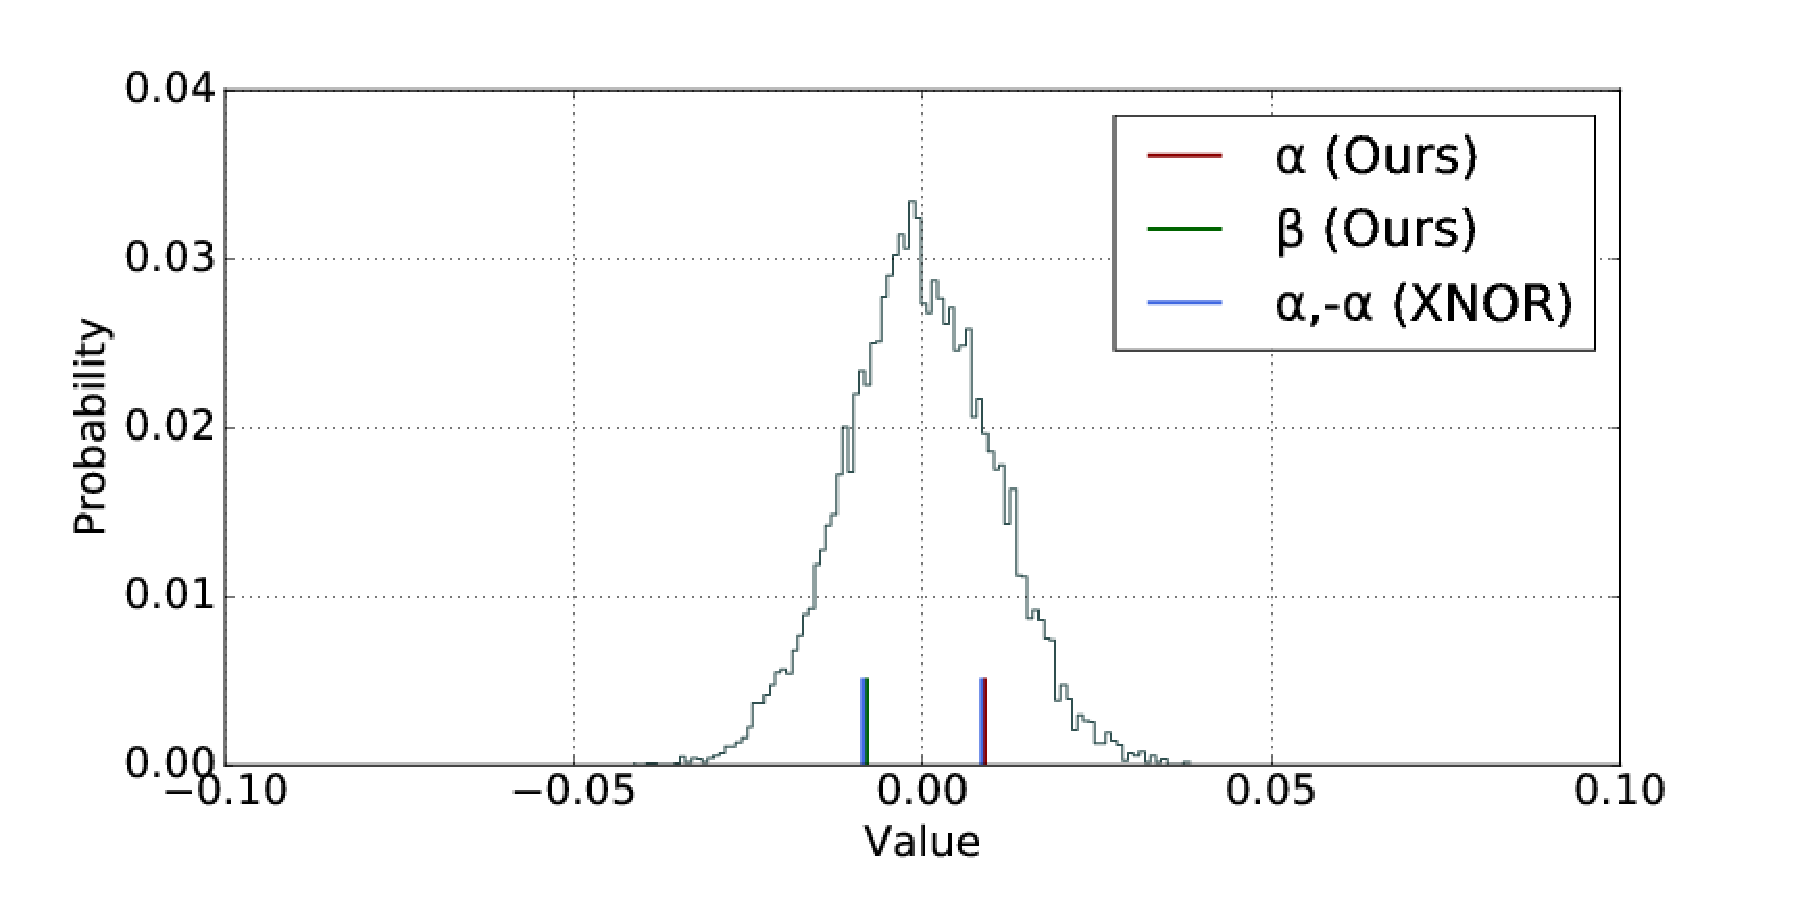
\includegraphics[page=1,width=0.5\columnwidth]{figures/figure21222324.pdf} & 
           \includegraphics[page=2,width=0.5\columnwidth]{figures/figure21222324.pdf}\\
           (1) & (2)\\
           \includegraphics[page=3,width=0.5\columnwidth]{figures/figure21222324.pdf} & \includegraphics[page=4,width=0.5\columnwidth]{figures/figure21222324.pdf}\\
           (3) & (4)\\  
\end{tabular}
\end{center}
\caption{Sub-figures (1) to (4) show the train-time variation of $\alpha$ and $\beta$ for a layer filter. Initially, $\alpha$ and $\beta$ have nearly equal magnitudes, similar to the XNOR-Net formulation, but as we progress to (4), we see that $\alpha$ and $\beta$ have widely different magnitudes.% and an approximation with only one scaling constant would be off compared to our $\alpha$-$\beta$ approximation.
Having just one scaling constant (XNOR-Net) would be a comparatively poor approximator.}
        \label{fig:alphabetaovertime}
\end{figure*}
\begin{figure*}[t]
\begin{center}
\begin{tabular}{cc}
           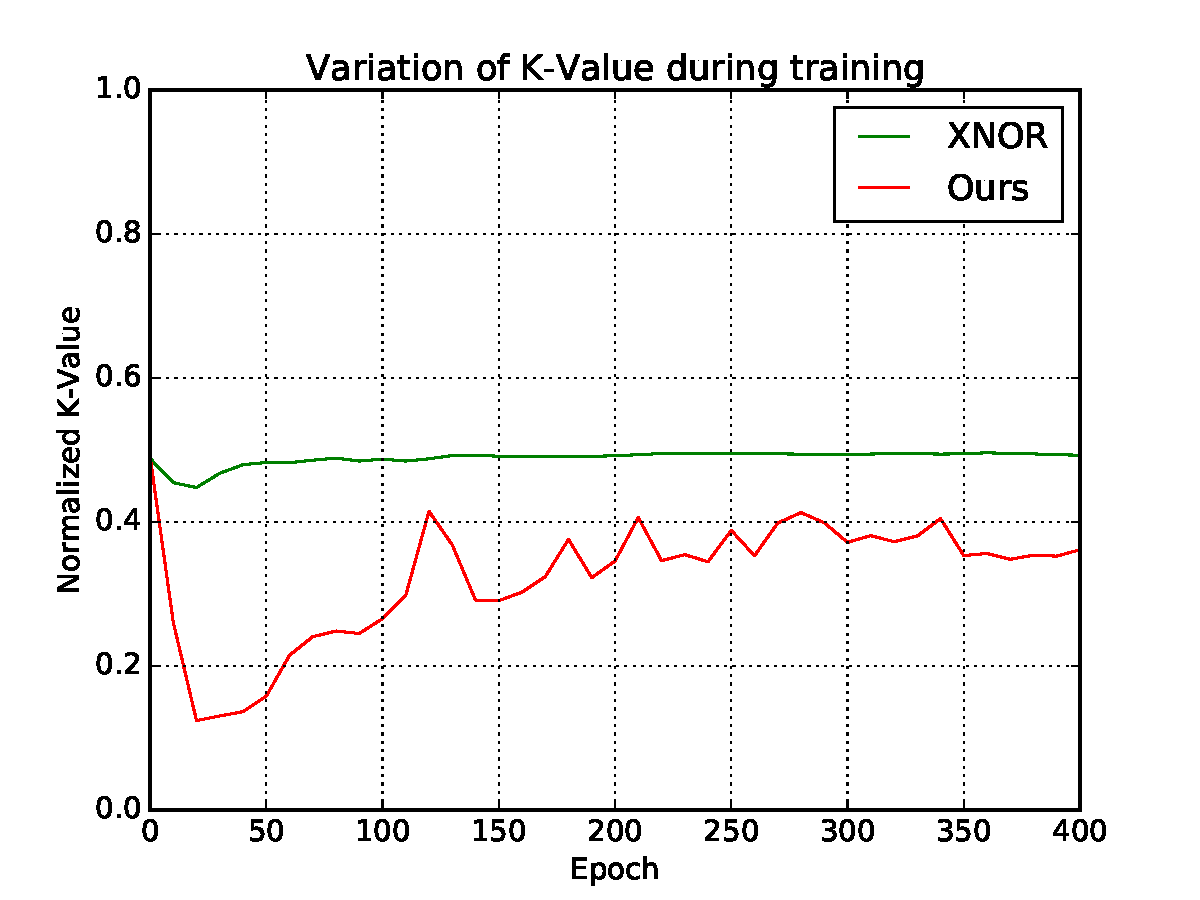
\includegraphics[width=0.5\textwidth]{figures/figure_1.pdf} & 
           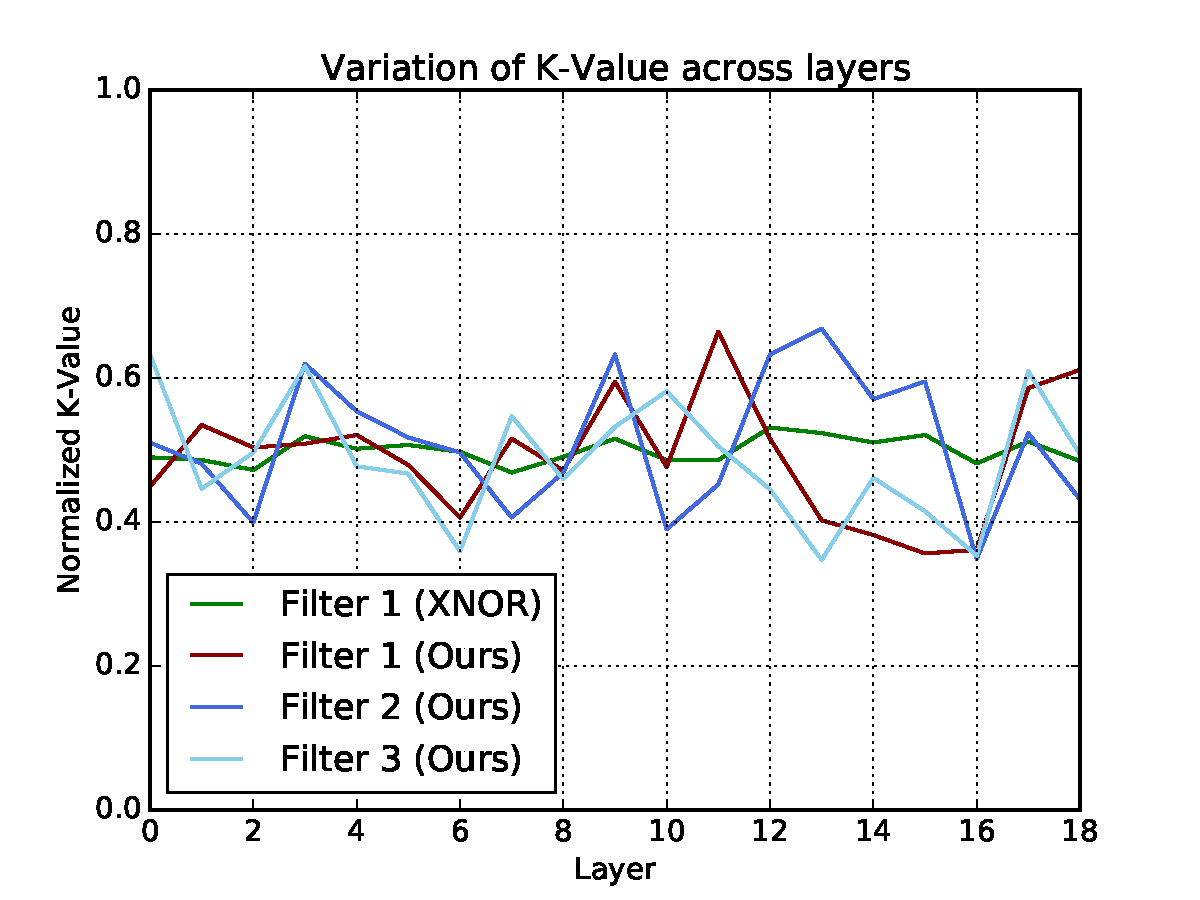
\includegraphics[width=0.5\textwidth]{figures/figure_3.pdf}\\
           (1) & (2)\\ 
\end{tabular}
\end{center}
\caption{(1) shows the variation of the normalized K-value over time during training. It falls initially but converges eventually to 0.35. The normalized K-value for XNOR-Net remains almost at 0.5 till the end. (2) shows the variation of normalized K values on random filters across layers. The K-value corresponding to DAB-Net varies across layers based on the distribution of weights of the specific layer, which is not captured by XNOR-Net.}
        \label{fig:alphabetaovertime}
\end{figure*}

\subsection{Results}

\noindent We compare the accuracies of our distribution aware binarization algorithm for WBin and FBin models on the TU-Berlin and Sketchy datasets. Note that higher accuracies are an improvement, hence stated in green in Table \ref{table:tub_recacc}. \\

\noindent On the TU-Berlin and Sketchy datasets in Table \ref{table:tub_recacc}, we observe that FBin DAB-Net models consistently perform better over their XNOR-Net counterparts. They improve upon XNOR-Net accuracies by 0.8\%, 2.5\%, and 1.5\% in Sketch-A-Net, ResNet-18, and GoogleNet respectively on the TU-Berlin dataset. Similarly, they improve by 2.0\%, 1.4\%, and 0.6\% respectively on the Sketchy dataset. We also compare them with state-of-the-art sketch classification models in Table \ref{table:sketchcomp}. We find that our compressed models perform significantly better than the original sketch models and offer compression, runtime and energy savings additionally.




\footnotetext{It is the sketch-a-net SC model trained with additional imagenet data, additional data augmentation strategies and considering an ensemble, hence would not be a direct comparison}

\noindent Our DAB-Net WBin models attain accuracies similar to BWN WBin models and do not offer major  improvements mainly because WBin models achieve FPrec accuracies already, hence do not have much scope for improvement unlike FBin models. Thus, we conclude that our DAB-Net FBin models are able to attain significant accuracy improvements over their XNOR-Net counterparts when everything apart from the binarization method is kept constant.


\subsection{XNOR-Net vs DAB-Net}

\noindent We measure how $K$, $\alpha$, and $\beta$ vary across various layers over time during training, and these variations are observed to be quite different from their corresponding values in XNOR-Net. These observations show that binarization can approximate a network much better when it is distribution-aware (like in our technique) versus when it is distribution-agnostic (like XNOR-Nets).

\subsubsection{Variation of $\alpha$ and $\beta$ across Time}

\noindent We plot the distribution of weights of a randomly selected filter belonging to a layer and observe that $\alpha$ and $\beta$ of DAB-Net start out to be similar to $\alpha$ and $-\alpha$ of XNOR-Nets, since the distributions are randomly initialized. However, as training progresses, we observe as we go from Subfigure (1) to (4) in Figure \ref{fig:alphabetaovertime}, the distribution eventually becomes non-symmetric and complex, hence our values  significantly diverge from their XNOR-Net counterparts. This divergence signifies a better approximation of the underlying distribution of weights in our method, giving additional evidence to our claim that the proposed DAB-Net technique gives a better representation of layer weights, significantly different from that of XNOR-Nets.

\subsubsection{Variation of $K$ across Time and Layers}\label{sec:kacrosslayers}

\noindent We define \textit{normalized} $K$ as the $\frac{K}{n}$ for a layer filter. For XNOR-Nets, $K$ would be the number of values below zero in a given weight filter - which has minimal variation, and does not take into consideration the distribution of weights in the filter - as $K$ in this case is simply the number of weights below a certain fixed global threshold, zero. However, we observe that the $K$ computed in DAB-Net varies significantly across epochs initially, but slowly converges to an optimal value for the specific layer as shown in Figure \ref{fig:alphabetaovertime}.\\

\noindent We also plot the variation of \textit{normalized} $K$ values for a few randomly chosen filters indexes across layers and observe that it varies across layers, trying to match the distribution of weights at each layer. Each filter has its own set of weights, accounting for the differences in variation of $K$ in each case, as shown in Figure \ref{fig:alphabetaovertime}.

\section{Summary}

\noindent We have proposed an optimal binary representation for network layer-weights that takes into account the distribution of weights, unlike previous distribution-agnostic approaches. We showed how this representation could be computed efficiently in $n.logn$ time using dynamic programming, thus enabling efficient training on larger datasets. We applied our technique on various datasets and noted significant accuracy improvements over other full-binarization approaches. 